\addtocontents{toc}{\vspace{2em}}
\chapter{Το Liqueur Plant Σύστημα Παραγωγής} % Main chapter title

\label{Chapter5} 

Στο [56] περιγράφεται ένα σύστημα παραγωγής liqueur και ένα σύστημα ελέγχου του βιομηχανικού συστήματος παραγωγής, βασισμένο σε PLC’s προγραμματισμένα σε γλώσσες προτύπου IEC61131. Στα πλαίσια της παρούσας διπλωματικής εργασίας αναπτύχθηκε για το ίδιο σύστημα παραγωγής ένα σύστημα ελέγχου βασισμένο σε τεχνολογίες ΙοΤ ακολουθώντας την component-based προσέγγιση για την ανάπτυξη του λογισμικού. Στο εξής θα γίνονται αναφορές σε αυτό το βιομηχανικό σύστημα παραγωγής σαν LPPS. Το συγκεκριμένο βιομηχανικό σύστημα έχει μελετηθεί ήδη και στις [57], [58], [59]. Έτσι μελετήθηκε, σχεδιάστηκε και υλοποιήθηκε ένα σύστημα παραγωγής  δύο τύπων liqueur βασισμένο στις προδιαγραφές του LPPS, το οποίο φαίνεται στην εικόνα 5.1:


\begin{figure}[htbp]
	\centering
		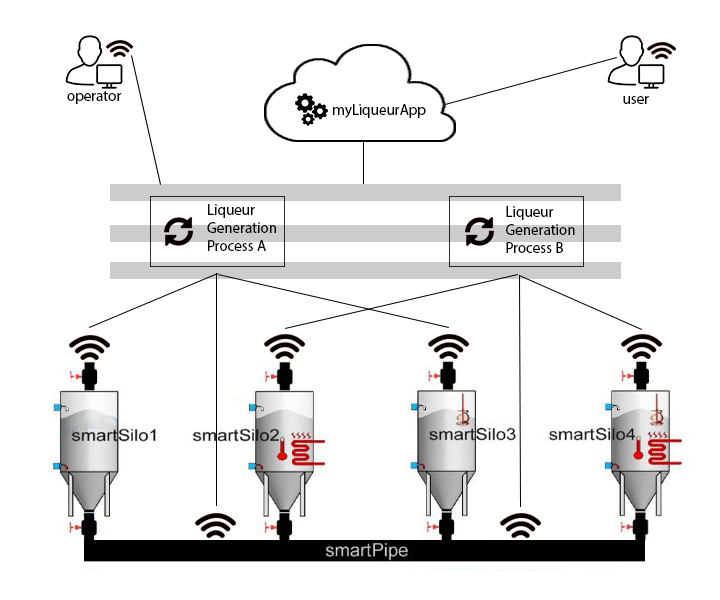
\includegraphics[height=11cm,width=15cm]{Figures/11.png}
	\caption{Σχηματική αναπαράσταση του συστήματος παραγωγής liqueur \cite{Thrampo3} }	
\end{figure}


	Το σύστημα αποτελείται από τέσσερα σιλό συνδεδεμένα μεταξύ τους με ένα σωλήνα. Κάθε ένα σιλό αποτελείται από μία βαλβίδα εισαγωγής και μία βαλβίδα εξαγωγής υγρού, καθώς και από δύο αισθητήρες για τον έλεγχο της παρουσίας υγρού, έναν στο πάνω μέρος ο οποίος ανιχνεύει αν το σιλό έχει γεμίσει  και έναν στο κάτω μέρος που ανιχνεύει αν το σιλό έχει αδειάσει. Επιπλέον, δύο από τα σιλό, το smartSilo2 και το smartSilo4, έχουν ένα στοιχείο θέρμανσης του υγρού και έναν αισθητήρα που ανιχνεύει την θερμοκρασία του υγρού. Τα smartSilo3 και smartSilo4 περιλαμβάνουν από ένα στοιχείο μίξης του υγρού. 

	Στο συγκεκριμένο σύστημα παράγονται δύο τύποι liqueur ακολουθώντας την εξής διαδικασία: 

\begin{itemize}
	\item{\textbf{Παραγωγή τύπου liqueur A}: Για να ξεκινήσει η παραγωγή του liqueur τύπου Α, το σιλό 1 γεμίζει με υγρό. Μόλις γεμίσει θα πρέπει να μεταφερθεί το υγρό αυτό μέσω του σωλήνα στο σιλό 4. Στη συνέχεια μόλις μεταφερθεί όλο το υγρό στο σιλό 4, θερμαίνεται μέχρι να φτάσει σε μία επιθυμητή θερμοκρασία και τέλος αναδεύεται για ένα συγκεκριμένο χρονικό διάστημα με την χρήση του στοιχείου μίξης του σιλό 4. Τέλος το υγρό μεταφέρεται σε άλλο σημείο παραγωγής μέσω της βαλβίδας εξαγωγής του σιλό 4. }
	\item{\textbf{Παραγωγή τύπου liqueur B}: Για την παραγωγή liqueur τύπου Β το σιλό 2 γεμίζει με υγρό. Μόλις γεμίσει το υγρό θερμαίνεται μέχρι να φτάσει σε μία επιθυμητή θερμοκρασία. Στη συνέχεια θα πρέπει να μεταφερθεί μέσω του σωλήνα στο σιλό 3. Αφού μεταφερθεί το υγρό αναδεύεται για ένα συγκεκριμένο χρονικό διάστημα μέσω του στοιχείου μείξης του σιλό 3. Τέλος, το υγρό μεταφέρεται σε άλλο σημείο παραγωγής μέσω της βαλβίδας εξαγωγής του σιλό 3. }
\end{itemize}

Οι δύο τύποι liqueur που μπορούν να παραχθούν καθώς και η διαδικασίες που ακολουθούνται για την παραγωγή τους είναι ανεξάρτητες και μπορούν να γίνουν ταυτόχρονα. Αλλά θα πρέπει να ληφθούν υπόψιν οι εξής περιορισμοί. Ο σωλήνας είναι κοινός πόρος και μπορεί να υποστηρίξει μία μεταφορά κάθε φορά. Δηλαδή μεταφορά υγρού από το σιλό 1 στο σιλό 4 ή μεταφορά υγρού από το σιλό 2 στο σιλό 3. Επιπλέον, υπάρχει και περιορισμός στην κατανάλωση ισχύος και γι’ αυτό θα πρέπει να λειτουργεί μόνο ένας αναδευτήρας κάθε φορά και όχι και οι δύο ταυτόχρονα. 

Οποιοσδήποτε χρήστης του myLiqueurApp θα μπορεί να ορίζει τον τύπο του liqueur που θέλει καθώς και τις διάφορες ιδιότητες του, δηλαδή σε ποια θερμοκρασία πρέπει να θερμανθεί και για πόση ώρα θα πρέπει να αναδευτεί καθώς και την ποσότητα που θέλει. Επιπλέον, θεωρούμε ότι τα σιλό απέχουν αρκετά μεταξύ τους ώστε να έχει σημασία η χρήση τεχνολογιών IoT για την επικοινωνία τους.